\documentclass[10pt,twoside]{article}

\newcommand{\reporttitle}{Levels 1-4}
\newcommand{\reportauthora}{Ayush Bansal}
\newcommand{\reportauthorb}{Gunjan Jalori}
\newcommand{\reportauthorc}{Siddharth Nohria}
\newcommand{\reporttype}{Solutions Report}
\newcommand{\cida}{160177}
\newcommand{\cidb}{170283}
\newcommand{\cidc}{160686}

% include files that load packages and define macros
%%%%%%%%%%%%%%%%%%%%%%%%%%%%%%%%%%%%%%%%%
% University Assignment Title Page 
% LaTeX Template
% Version 1.0 (27/12/12)
%
% This template has been downloaded from:
% http://www.LaTeXTemplates.com
%
% Original author:
% WikiBooks (http://en.wikibooks.org/wiki/LaTeX/Title_Creation)
%
% License:
% CC BY-NC-SA 3.0 (http://creativecommons.org/licenses/by-nc-sa/3.0/)
% 
% Instructions for using this template:
% This title page is capable of being compiled as is. This is not useful for 
% including it in another document. To do this, you have two options: 
%
% 1) Copy/paste everything between \begin{document} and \end{document} 
% starting at \begin{titlepage} and paste this into another LaTeX file where you 
% want your title page.
% OR
% 2) Remove everything outside the \begin{titlepage} and \end{titlepage} and 
% move this file to the same directory as the LaTeX file you wish to add it to. 
% Then add \input{./title_page_1.tex} to your LaTeX file where you want your
% title page.
%
%----------------------------------------------------------------------------------------
%	PACKAGES AND OTHER DOCUMENT CONFIGURATIONS
%----------------------------------------------------------------------------------------
\usepackage{ifxetex}
\usepackage{textpos}
\usepackage{natbib}
\usepackage{kpfonts}
\usepackage[a4paper,hmargin=2.8cm,vmargin=2.0cm,includeheadfoot]{geometry}
\usepackage{ifxetex}
\usepackage{stackengine}
\usepackage{tabularx,longtable,multirow,subfigure,caption}%hangcaption
\usepackage{fncylab} %formatting of labels
\usepackage{fancyhdr}
\usepackage{color}
\usepackage[tight,ugly]{units}
\usepackage{url}
\usepackage{float}
\usepackage[english]{babel}
\usepackage{amsmath}
\usepackage{graphicx}
\usepackage[colorinlistoftodos]{todonotes}
\usepackage{dsfont}
\usepackage{epstopdf} % automatically replace .eps with .pdf in graphics
\usepackage{natbib}
\usepackage{backref}
\usepackage{array}
\usepackage{latexsym}
\usepackage{etoolbox}

\usepackage{enumerate} % for numbering with [a)] format 

\usepackage{minted}

\ifxetex
\usepackage{fontspec}
\else
\usepackage[pdftex,pagebackref,hypertexnames=false,colorlinks]{hyperref} % provide links in pdf
\hypersetup{pdftitle={},
  pdfsubject={}, 
  pdfauthor={\reportauthora \newline \reportauthorb \newline \reportauthorc},
  pdfkeywords={}, 
  pdfstartview=FitH,
  pdfpagemode={UseOutlines},% None, FullScreen, UseOutlines
  bookmarksnumbered=true, bookmarksopen=true, colorlinks,
    citecolor=black,%
    filecolor=black,%
    linkcolor=black,%
    urlcolor=black}
\usepackage[all]{hypcap}
\fi

\usepackage{tcolorbox}

% various theorems
\usepackage{ntheorem}
\theoremstyle{break}
\newtheorem{lemma}{Lemma}
\newtheorem{theorem}{Theorem}
\newtheorem{remark}{Remark}
\newtheorem{definition}{Definition}
\newtheorem{proof}{Proof}

% example-environment
\newenvironment{example}[1][]
{ 
\vspace{4mm}
\noindent\makebox[\linewidth]{\rule{\hsize}{1.5pt}}
\textbf{Example #1}\\
}
{ 
\noindent\newline\makebox[\linewidth]{\rule{\hsize}{1.0pt}}
}



%\renewcommand{\rmdefault}{pplx} % Palatino
% \renewcommand{\rmdefault}{put} % Utopia

\ifxetex
\else
\renewcommand*{\rmdefault}{bch} % Charter
\renewcommand*{\ttdefault}{cmtt} % Computer Modern Typewriter
%\renewcommand*{\rmdefault}{phv} % Helvetica
%\renewcommand*{\rmdefault}{iwona} % Avant Garde
\fi

\setlength{\parindent}{0em}  % indentation of paragraph

\setlength{\headheight}{14.5pt}
\pagestyle{fancy}
\fancyfoot[ER,OL]{\thepage}%Page no. in the left on
                                %odd pages and on right on even pages
\fancyfoot[OC,EC]{\sffamily }
\renewcommand{\headrulewidth}{0.1pt}
\renewcommand{\footrulewidth}{0.1pt}
\captionsetup{margin=10pt,font=small,labelfont=bf}


%--- chapter heading

\def\@makechapterhead#1{%
  \vspace*{10\p@}%
  {\parindent \z@ \raggedright %\sffamily
        %{\Large \MakeUppercase{\@chapapp} \space \thechapter}
        %\\
        %\hrulefill
        %\par\nobreak
        %\vskip 10\p@
    \interlinepenalty\@M
    \Huge \bfseries 
    \thechapter \space\space #1\par\nobreak
    \vskip 30\p@
  }}

%---chapter heading for \chapter*  
\def\@makeschapterhead#1{%
  \vspace*{10\p@}%
  {\parindent \z@ \raggedright
    \sffamily
    \interlinepenalty\@M
    \Huge \bfseries  
    #1\par\nobreak
    \vskip 30\p@
  }}
  



% %%%%%%%%%%%%% boxit
\def\Beginboxit
   {\par
    \vbox\bgroup
	   \hrule
	   \hbox\bgroup
		  \vrule \kern1.2pt %
		  \vbox\bgroup\kern1.2pt
   }

\def\Endboxit{%
			      \kern1.2pt
		       \egroup
		  \kern1.2pt\vrule
		\egroup
	   \hrule
	 \egroup
   }	

\newenvironment{boxit}{\Beginboxit}{\Endboxit}
\newenvironment{boxit*}{\Beginboxit\hbox to\hsize{}}{\Endboxit}



\allowdisplaybreaks

\makeatletter
\newcounter{elimination@steps}
\newcolumntype{R}[1]{>{\raggedleft\arraybackslash$}p{#1}<{$}}
\def\elimination@num@rights{}
\def\elimination@num@variables{}
\def\elimination@col@width{}
\newenvironment{elimination}[4][0]
{
    \setcounter{elimination@steps}{0}
    \def\elimination@num@rights{#1}
    \def\elimination@num@variables{#2}
    \def\elimination@col@width{#3}
    \renewcommand{\arraystretch}{#4}
    \start@align\@ne\st@rredtrue\m@ne
}
{
    \endalign
    \ignorespacesafterend
}
\newcommand{\eliminationstep}[2]
{
    \ifnum\value{elimination@steps}>0\leadsto\quad\fi
    \left[
        \ifnum\elimination@num@rights>0
            \begin{array}
            {@{}*{\elimination@num@variables}{R{\elimination@col@width}}
            |@{}*{\elimination@num@rights}{R{\elimination@col@width}}}
        \else
            \begin{array}
            {@{}*{\elimination@num@variables}{R{\elimination@col@width}}}
        \fi
            #1
        \end{array}
    \right]
    & 
    \begin{array}{l}
        #2
    \end{array}
    &%                                    moved second & here
    \addtocounter{elimination@steps}{1}
}
\makeatother

%% Fast macro for column vectors
\makeatletter  
\def\colvec#1{\expandafter\colvec@i#1,,,,,,,,,\@nil}
\def\colvec@i#1,#2,#3,#4,#5,#6,#7,#8,#9\@nil{% 
  \ifx$#2$ \begin{bmatrix}#1\end{bmatrix} \else
    \ifx$#3$ \begin{bmatrix}#1\\#2\end{bmatrix} \else
      \ifx$#4$ \begin{bmatrix}#1\\#2\\#3\end{bmatrix}\else
        \ifx$#5$ \begin{bmatrix}#1\\#2\\#3\\#4\end{bmatrix}\else
          \ifx$#6$ \begin{bmatrix}#1\\#2\\#3\\#4\\#5\end{bmatrix}\else
            \ifx$#7$ \begin{bmatrix}#1\\#2\\#3\\#4\\#5\\#6\end{bmatrix}\else
              \ifx$#8$ \begin{bmatrix}#1\\#2\\#3\\#4\\#5\\#6\\#7\end{bmatrix}\else
                 \PackageError{Column Vector}{The vector you tried to write is too big, use bmatrix instead}{Try using the bmatrix environment}
              \fi
            \fi
          \fi
        \fi
      \fi
    \fi
  \fi 
}  
\makeatother

\robustify{\colvec}

%%% Local Variables: 
%%% mode: latex
%%% TeX-master: "notes"
%%% End: 
 % various packages needed for maths etc.
% quick way of adding a figure
\newcommand{\fig}[3]{
 \begin{center}
 \scalebox{#3}{\includegraphics[#2]{#1}}
 \end{center}
}

%\newcommand*{\point}[1]{\vec{\mkern0mu#1}}
\newcommand{\ci}[0]{\perp\!\!\!\!\!\perp} % conditional independence
\newcommand{\point}[1]{{#1}} % points 
\renewcommand{\vec}[1]{{\boldsymbol{{#1}}}} % vector
\newcommand{\mat}[1]{{\boldsymbol{{#1}}}} % matrix
\newcommand{\R}[0]{\mathds{R}} % real numbers
\newcommand{\Z}[0]{\mathds{Z}} % integers
\newcommand{\N}[0]{\mathds{N}} % natural numbers
\newcommand{\nat}[0]{\mathds{N}} % natural numbers
\newcommand{\Q}[0]{\mathds{Q}} % rational numbers
\ifxetex
\newcommand{\C}[0]{\mathds{C}} % complex numbers
\else
\newcommand{\C}[0]{\mathds{C}} % complex numbers
\fi
\newcommand{\tr}[0]{\text{tr}} % trace
\renewcommand{\d}[0]{\mathrm{d}} % total derivative
\newcommand{\inv}{^{-1}} % inverse
\newcommand{\id}{\mathrm{id}} % identity mapping
\renewcommand{\dim}{\mathrm{dim}} % dimension
\newcommand{\rank}[0]{\mathrm{rk}} % rank
\newcommand{\determ}[1]{\mathrm{det}(#1)} % determinant
\newcommand{\scp}[2]{\langle #1 , #2 \rangle}
\newcommand{\kernel}[0]{\mathrm{ker}} % kernel/nullspace
\newcommand{\img}[0]{\mathrm{Im}} % image
\newcommand{\idx}[1]{{(#1)}}
\DeclareMathOperator*{\diag}{diag}
\newcommand{\E}{\mathds{E}} % expectation
\newcommand{\var}{\mathds{V}} % variance
\newcommand{\gauss}[2]{\mathcal{N}\big(#1,\,#2\big)} % gaussian distribution N(.,.)
\newcommand{\gaussx}[3]{\mathcal{N}\big(#1\,|\,#2,\,#3\big)} % gaussian distribution N(.|.,.)
\newcommand{\gaussBig}[2]{\mathcal{N}\left(#1,\,#2\right)} % see above, but with brackets that adjust to the height of the arguments
\newcommand{\gaussxBig}[3]{\mathcal{N}\left(#1\,|\,#2,\,#3\right)} % see above, but with brackets that adjust to the height of the arguments
\newcommand{\matdet}[1]{
\left|
\begin{matrix}
#1
\end{matrix}
\right|
}



%%% various color definitions
\definecolor{darkgreen}{rgb}{0,0.6,0}

\newcommand{\blue}[1]{{\color{blue}#1}}
\newcommand{\red}[1]{{\color{red}#1}}
\newcommand{\green}[1]{{\color{darkgreen}#1}}
\newcommand{\orange}[1]{{\color{orange}#1}}
\newcommand{\magenta}[1]{{\color{magenta}#1}}
\newcommand{\cyan}[1]{{\color{cyan}#1}}


% redefine emph
\renewcommand{\emph}[1]{\blue{\bf{#1}}}

% place a colored box around a character
\gdef\colchar#1#2{%
  \tikz[baseline]{%
  \node[anchor=base,inner sep=2pt,outer sep=0pt,fill = #2!20] {#1};
    }%
}%
 % short-hand notation and macros

%\setlength{\parskip}{0pt}
%\setlength{\parsep}{0pt}
%\setlength{\topskip}{0pt}
%\setlength{\topmargin}{0pt}
%\setlength{\partopsep}{0pt}
%%\setlength\lineskip{0pt}
%\linespread{0.5}
%\setlength{\textfloatsep}{2pt}
%\setlength{\intextsep}{2pt}

%\setlength\itemsep{0em}

\newcommand{\myth}[1]{\textcolor{red}{\hl{#1}}}

%%%%%%%%%%%%%%%%%%%%%%%%%%%%

\begin{document}
% front page
% Last modification: 2016-09-29 (Marc Deisenroth)
\begin{titlepage}

\newcommand{\HRule}{\rule{\linewidth}{0.5mm}} % Defines a new command for the horizontal lines, change thickness here


%----------------------------------------------------------------------------------------
%	LOGO SECTION
%----------------------------------------------------------------------------------------

\begin{center} % Center remainder of the page

%----------------------------------------------------------------------------------------
%	HEADING SECTIONS
%----------------------------------------------------------------------------------------
\textsc{\LARGE \reporttype}\\[1.5cm] 
\textsc{\Large Modern Cryptology (CS641)}\\[0.5cm]
\textsc{\large Computer Science and Engineering}\\[0.5cm] 
%----------------------------------------------------------------------------------------
%	TITLE SECTION
%----------------------------------------------------------------------------------------

\HRule \\[0.4cm]
{ \huge \bfseries \reporttitle}\\ % Title of your document
\HRule \\[1.5cm]
\end{center}
%----------------------------------------------------------------------------------------
%	AUTHOR SECTION
%----------------------------------------------------------------------------------------

%\begin{minipage}{0.4\hsize}
\begin{flushleft} \large
\textit{Team:} \textbf{team58}\\
\reportauthora~(\cida)\\
\reportauthorb~(\cidb)\\
\reportauthorc~(\cidc)\\
\vspace{1cm}
\end{flushleft}
\vspace{2cm}
\makeatletter
Date: \@date 

\vfill % Fill the rest of the page with whitespace



\makeatother


\end{titlepage}



%%%%%%%%%%%%%%%%%%%%%%%%%%%% Main document
\section{Chapter 1 (The Entry)}

There are 5 sub-levels in the chapter, first 4 of these don't have any cipher which needs to be decrypted. \newline

The last sub-level is a \textbf{Substitution Cipher}, the answer to - ``how it was recognised and solved" is explained in the subsection after the following list of commands. \newline

Below is the solution to each of the sub-levels:
\begin{enumerate}
  \setlength\itemsep{0em}
  \item go
  \item read
  \item enter
  \item read
  \item cyLe70Lecy
\end{enumerate}

\subsection{Substitution Cipher}

The ciphertext given was: \newline

\texttt{Nwy dejp pmcplpz cdp sxlrc adegipl ws cdp aejpr. Er nwy aem rpp cdplp xr mwcdxmv ws xmcplprc xm cdp adegipl. Rwgp ws cdp qecpl adegiplr fxqq ip gwlp xmcplprcxmv cdem cdxr wmp, x eg rplxwyr. Cdp awzp yrpz swl cdxr gprrevp xr e rxgbqp ryircxcycxwm axbdpl xm fdxad zxvxcr dejp ippm rdxscpz in 2 bqeapr. Swl cdxr lwymz berrfwlz xr vxjpm ipqwf, fxcdwyc cdp hywcpr.} \newline

For identifying what kind of cipher is applied in the above text, we will use the \textbf{Index of Coincidence}. \newline

The detailed explanation on \textit{Index of Coincidence} can be found in \cref{ic}. \newline

The \textit{Index of Coincidence} of the above ciphertext is about $0.07$, which is approximately same as a valid English text, this suggests that the cipher used is \textit{Mono-alphabetic} such as \textit{Substitution Cipher}. \newline

For Solving the \textit{Substitution Cipher}, the following steps were employed:
\begin{enumerate}
  \setlength\itemsep{0em}
    \item Calculate the frequency of each of the characters in the ciphertext, ignoring anything which is not an english alphabet.
    \item The Character with the highest frequency is most probably `e' or `a', which can be placed in its place and identified further.
    \item As the places get revealed, played hangman to find out what the other characters might be looking at one-letter, 2-letter, 3-letter words with highest number of characters revealed.
    \item Built the decryption key by keeping a map of characters as they are being replaced.
    \item Finally used the decryption key to decrypt the code given for the solution.
\end{enumerate}

The code used in this part is in the file - \texttt{break\_substitution.py}. \newline

The Steps employed in the hangman game and building the key are mentioned below:
\begin{minted}{python}
key = {}
key['p'] = 'e'    # Because 'p' has very high frequency
key['r'] = 's'    # 'r' has very high frequency,
                  #  _ee word exists, matches with "see" not "bee"
key['i'] = 'b'    # _e word exists, matches with "be"
key['n'] = 'y'    # b_ word exists, matches with "by"
key['m'] = 'n'    # bee_ word exists, matches with "been"
key['w'] = 'o'    # _ne word exists, matches with "one"
key['s'] = 'f'    # o_ word exists, 'n' is already taken, matches with "of"
key['l'] = 'r'    # fo_ word exists, matches with "for"
key['y'] = 'u'    # yo_ word exists, matches with "you"
key['g'] = 'm'    # so_e word exists, matches with "some"
key['z'] = 'd'    # use_ word exists, 'r' is already taken, matches with "used"
key['c'] = 't'    # en_ered word exists, matches with "entered"
key['d'] = 'h'    # t_e word exists, matches with "the"
key['x'] = 'i'    # f_rst word and _ (single letter word) exist,
                  # matches with "first" and "i"
key['e'] = 'a'    # single letter word exists, 'i' is already taken, matches with "a"
key['j'] = 'v'    # ha_e word exists, matches with "have"
key['a'] = 'c'    # _hamber word exists, matches with "chamber"
key['v'] = 'g'    # nothin_ word exists, matches with "nothing"
key['f'] = 'w'    # _hich word exists, matches with "which"
key['q'] = 'l'    # be_ow and wi__ word exists, matches with "below" and "will"
key['b'] = 'p'    # sim_le and ci_her word exists, matches with "simple" and "cipher"
key['h'] = 'q'    # _uotes word exists, matches with "quotes"
\end{minted}

The plaintext revealed after using the above decryption key is: \newline

\texttt{You  have  entered  the  first  chamber  of  the  caves.  As  you  can  see  there  is  nothing  of  interest  in  the  chamber.  Some  of  the  later  chambers  will  be  more  interesting  than  this  one,  i  am  serious.  The  code  used  for  this  message  is  a  simple  substitution  cipher  in  which  digits  have  been  shifted  by  2  places.  For  this  round  password  is  given  below,  without  the  quotes.}

\begin{minted}{python}
# For the case of integer digits, "1" must be subtracted from each digit, as mentioned
# text after decryption, it was "2" but it itself was shifted so
# x+x = 2, this gives x = 1
\end{minted}

So, final plaintext is: \newline

\texttt{You  have  entered  the  first  chamber  of  the  caves.  As  you  can  see  there  is  nothing  of  interest  in  the  chamber.  Some  of  the  later  chambers  will  be  more  interesting  than  this  one,  i  am  serious.  The  code  used  for  this  message  is  a  simple  substitution  cipher  in  which  digits  have  been  shifted  by  1  places.  For  this  round  password  is  given  below,  without  the  quotes.} \newline

Using the above decryption key and the logic for digit, we can decipher the code for the answer as well: \newline

Code: \texttt{anQp81Qpan} \newline
Solution: \texttt{cyLe70Lecy}
\newpage
\section{Chapter 2 (The Caveman)}
There are 2 sub-levels in the chapter, first one doesn't have any cipher which needs to be decrypted. \newline

The second sub-level is a \textbf{Vigenere Cipher}, the answer to - ``how it was recognised and solved" is explained in the subsection after the following list of commands. \newline

The detailed explanation on \textit{Vigenere Cipher} can be found in \cref{vc}. \newline

Below is the solution to each of the sub-levels:
\begin{enumerate}
  \setlength\itemsep{0em}
    \item read
    \item the\_cave\_man\_be\_pleased
\end{enumerate}

\subsection{Vigenere Cipher}
The ciphertext given was: \newline

\texttt{Lg ccud qh urg tgay ejbwdkt, wmgtf su bgud nkudnk lrd vjfbg. Yrhfm qvd vng sfuuxytj \newline "vkj\_ecwo\_ogp\_ej\_rnfkukf" wt iq urtuwjm. Ocz iqa jdag vio uzthsivi pqx vkj pgyd encpggt. Uy hopg yjg fhkz arz hkscv ckoq pgfn vu wwygt nkioe zttft djkth.} \newline

For identifying what kind of cipher is applied in the above text, we will use the \textbf{Index of Coincidence}. \newline

The detailed explanation on \textit{Index of Coincidence} can be found in \cref{ic}. \newline

The \textit{Index of Coincidence} of the above ciphertext is about $0.042$, which is closer to the uniform distribution of English text, this suggests that the cipher is \textit{Poly-alphabetic} such as \textit{Vigenere Cipher}, it may be some other Poly-alphabetic cipher as well but we still have to give it a shot. \newline

For solving the \textit{Vigenere Cipher}, the following steps were employed:
\begin{enumerate}
  \setlength\itemsep{0em}
    \item Remove all characters from the text which are not part of the English alphabets and capitilize all characters.
    \item Partition the text according to different key lengths and sort them according to the \textit{Index of Coincidences} achieved, since higher the IC, closer it is to valid English Text.
    \item For each keylen, perform frequency analysis to get the best key possible with the given length.
    \item Try out all the keys retrieved and see which one gives some valid English text.
\end{enumerate}

The code used in this part is in the file - \texttt{break\_vigenere.py}. \newline

The plaintext revealed after using the above decryption key is: \newline

\texttt{Be wary of the next chamber, there is very little joy there. Speak out the password \newline"the\_cave\_man\_be\_pleased" to go through. May you have the strength for the next chamber. To find the exit you first will need to utter magic words there.} \newline

From the above, the solution is revealed: \texttt{the\_cave\_man\_be\_pleased}.

\newpage
\section{Chapter 3 (The Holes)}
There are 4 sub-levels in the chapter, first 3 of these don't have any cipher but there are different tricks which need to be employed to get to the final sub-level. \newline

The last sub-level is a \textbf{Permutation-Substitution Cipher}, the answer to - ``how it was recognised and solved" is explained in the subsection after the following list of steps/commands. \newline

Below are the solution steps to get out of the final chamber:
\begin{enumerate}
  \setlength\itemsep{0em}
  \item Type \texttt{enter} to go to sub-level 2.
  \item At sub-level 2, you try to \texttt{put} your hand in the small hole, it is bitten, denoting there is someone there.
  \item Type \texttt{enter} to go to sub-level 3, here there are a lot of mushrooms growing on the ground.
  \item Type \texttt{pick} to pluck some mushrooms and come back to sub-level 2.
  \item Type \texttt{give} to give the mushrooms to whatever is there in the small hole.
  \item There is a spirit here, who gives you the code \texttt{thrnxxtzy} which can reveal a hidden door at the entrance chamber (sub-level 1).
  \item Go back to sub-level 1 and type \texttt{thrnxxtzy}, this reveals a hidden door with a glass panel beside it.
  \item Type \texttt{read} to get the ciphertext and code.
  \item Type \texttt{jyg\_izuqo\_rr}, which is the decoded plaintext from the cipher provided.
\end{enumerate}

\subsection{Permutation-Substitution Cipher}
The ciphertext given was: \newline

\texttt{cpiftgt ef oldo ukuq vtyp vv ptttqkk dp txe tkcnmbi uxkfft ueukwuqe ad uwv ttdo. da tocwc, qqc qgcu woyg cx cpifteud wat tvkbd vu owk zelc dp txe vthr uccfgg. keb dteuof ut gle dzcc rtc wv ukkyyc xxuo edw. mqgu zec dtyac uldw cqev evyu xvo tee moo mt gle dkcur. tm evyoi qtzc cxz o mlcuauoc, vw wetd kkcc gwhego! cf da foedokm, aibet ccd ktbfkqyo:} \newline

For identifying what kind of cipher is applied in the above text, we used the following techniques:

\begin{itemize}
  \setlength\itemsep{0em}
  \item The \textbf{Index of Coincidence} of the above ciphertext is about $0.057$, which is very close to that of valid English text, this suggests that the cipher used is \textit{Mono-alphabetic} such as \textit{Substitution Cipher}, the detailed explanation on \textit{Index of Coincidence} can be found in \cref{ic}.
  \item The \textbf{Chi-squared Statistic} of the above ciphertext is about $157$ against \textit{uniform distribution}, this suggests that the cipher used is \textit{not Poly-alphabetic} since it is not closer to uniform distribution, the detailed explanation on \textit{Chi-squared Statistic} can be found in \cref{chi}.
  \item The \textbf{Chi-squared Statistic} of the above ciphertext is about $958$ against \textit{valid English text}, this suggests that the cipher used is \textbf{not} a \textit{Simple Permutation} of letters.
  \item Based on the above, we try out different forms of \textit{Mono-alphabetic} ciphers first instead of \textit{Poly-alphabetic}.
\end{itemize}

Firstly, we will try to solve the cipher assuming it is \textit{Simple Substitution Cipher}. This doesn't seem to work, since we are not able to get any valid English text from it. \newline

The code for solving the Substitution Cipher uses the \textbf{n-gram} approach and it is in the file: \texttt{ngram\_score.py}. \newline

Since a \textit{Simple Substitution Cipher} doesn't work here, it could be some other form of \textit{Mono-alphabetic} cipher. \newline

Lets make some observations about the ciphertext:
\begin{itemize}
  \setlength\itemsep{0em}
    \item The occurrences of double letter phrases in words is very frequent and at very odd places, see the below text: \newline
      \texttt{cpiftgt ef oldo ukuq vtyp \myth{vv} p\myth{ttt}q\myth{kk} dp txe tkcnmbi uxk\myth{ff}t ueukwuqe ad uwv \myth{tt}do. da tocwc, \myth{qq}c qgcu woyg cx cpifteud wat tvkbd vu owk zelc dp txe vthr u\myth{cc}f\myth{gg}. keb dteuof ut gle dz\myth{cc} rtc wv u\myth{kkyy}c \myth{xx}uo edw. mqgu zec dtyac uldw cqev evyu xvo t\myth{ee} m\myth{oo} mt gle dkcur. tm evyoi qtzc cxz o mlcuauoc, vw wetd \myth{kkcc} gwhego! cf da foedokm, aibet \myth{cc}d ktbfkqyo:}
    \item The character `o' appears as a single letter, if we assume it to be `a' or `i' (according to english text), then the word `moo' will coincide to `\_aa' or `\_ii' which will not come out to be a valid English word.
    \item A simple substitution solver doesn't give us a valid result for the ciphertext.
\end{itemize}

The above observations suggest the following things:
\begin{itemize}
  \setlength\itemsep{0em}
    \item The letters in the ciphertext needs to be permuted before applying Substitution, this permutation can be a block permutation or matrix permutation or maybe something entirely different.
    \item The cipher is \textit{Poly-alphabetic} (less-likely).
\end{itemize}

Firstly, we will try out \textbf{block-permutation} along with \textbf{Substitution}, i.e. \textbf{Simple Permutation-Substitution Cipher}. \newline

For solving the \textit{Simple Permutation-Substitution Cipher}, the following steps were employed:
\begin{enumerate}
  \setlength\itemsep{0em}
    \item Remove all characters from the text which are not part of the English alphabets, noting their position in the text since they will have to be added back at the end.
    \item Calculate the \textit{block length} (for permutation) using the idea that block length will be a \textit{factor of the total number of characters}.
    \item For each permutation get the permutated text from the ciphertext, and insert all the special characters at their designated places in the text.
    \item Apply a Simple Substitution Cipher Solver to the text and see whether it gives a valid English Text.
    \item If no permutation gives a successful result, try other block length till we reach some valid English Text or run out of factors.
\end{enumerate}

The code used in this part is in the file - \texttt{break\_perm-subs.py}. \newline

The \textit{total number of characters} in the ciphertext is $270$.

Another observation to make here is that the code to be deciphered: \texttt{uhs\_xafmf\_no} has total of $10$ characters.

This suggests that the block length will be a factor of both $270$ and $10$, so it can be $2$, $5$ or $10$, and we will try each of these one by one. \newline

Using the method described above, we got each permutation of ciphertext corresponding to block-length $2$ first, but none of them returned a valid English text after solving the Substitution, so we changed block-length to $5$. \newline

Using block-length $5$ revealed the following plaintext after a certain permutation of ciphertext was solved using Substitution Cipher Solver: \newline

\texttt{breaker of this code will be blessed by the squeaky spirit residing in the hole. go ahead, and find away of breaking the spell on him cast by the evil jaffar. the spirit of the cave man is always with you. find the magic wand that will let you out of the caves. it would make you a magician, no less than jaffar! to go through, speak the password:} \newline

At this point, we got a valid English text from the ciphertext, so we won't be moving forward and trying out different block-length or other ciphers. \newline

Using the permutation and decryption key retrieved from solving above cipher, we can decipher the code for the answer as well: \newline

The decryption key retrieved from the Solver gave us $2$ possible solutions, since we did not have mapping for all $26$ characters: \newline
Code: \texttt{uhs\_xafmf\_no} \newline
Solution $1$: \texttt{jyg\_izuqo\_rr} \newline
Solution $2$: \texttt{jyg\_ixuqo\_rr} \newline

Finally, Solution $1$ was the answer.

\newpage
\section{Chapter 4 (The Spirit)}

This level is tricky as we had to go back to the previous level and perform some task before we could proceed further. \newline

There are 3 sub-tasks here, firstly we have to retrieve a \textit{Magic Wand}, secondly we have to \textit{free the Spirit}, finally solve the \textbf{DES Cipher} to advance to next level. \newline

Below are the solution steps for each of the tasks listed above:
\begin{itemize}
  \setlength\itemsep{0em}
  \item Retrieving the Magic Wand:
    \begin{enumerate}
      \item Type \texttt{enter} to go ahead in the chamber.
      \item Type \texttt{dive} to take a dive into the lake.
      \item At this point, we see an object looking like a wand, but trying to pull it directly causes us to drown, so first go back to surface and take a deep breath.
      \item Type \texttt{dive} and \texttt{pull} the wand.
    \end{enumerate}
  \item Freeing the Spirit:
    \begin{enumerate}
        \item At this point, we can't figure out any way out, the screen in the chamber door is also blank and wand does not help us here.
        \item We can recall that there was an old man/spirit before who helped us in chamber 3 and mentioned that he was trapped by someone, he could be freed by the magic wand.
        \item We go back to chamber 3, \texttt{wave} our wand infront of the hole where the old man's spirit was.
        \item The spirit is freed and says that he will help us along the way.
    \end{enumerate}
  \item Solving the \textbf{DES Cipher}:
    \begin{enumerate}
      \item After entering the 4th chamber, type \texttt{read}.
        \item The screen is still blank, but the spirit tells us what is supposed to be there: \newline
          \texttt{This is a magical screen. You can whisper something close to the screen and the corresponding coded text would appear on it after a while. So go ahead and try to break the code! The code used for this is a 4-round DES, so it should be easy for you!! Er wait ... maybe it is a 6-round DES ... sorry, my memory has blurred after so many years. But I am sure you can break even 6-round DES easily. A 10-round DES is a different matter, but this one surely is not 10-round ...(long pause) ... at least that is what I remember. One thing that I surely remember is that you can see the coded password by whispering 'password'. There was something funny about how the text appears, two letters for one byte or something like that. I do not recall more than that. I am sure you can figure it out though ...}
    \end{enumerate}
\end{itemize}

\subsection{3-Round DES Cipher}

Earlier, we were trying to figure out how many rounds of DES Cipher is applied here, so that we can devise the algorithm for the same. \newline

The task became easier when a hint was revealed stating that the DES Cipher is \textit{3 Round}. \newline

We will break \textit{3 Round DES} using \textbf{Differential Cryptanalysis} as we had discussed in class. \newline

The idea behind \textit{Differential Cryptanalysis} was to get rid of the unknown value (i.e. the Key) so that an equation can be formed over the non-linear step (i.e. sBoxes). \newline

\begin{figure}[H]
  \centering
  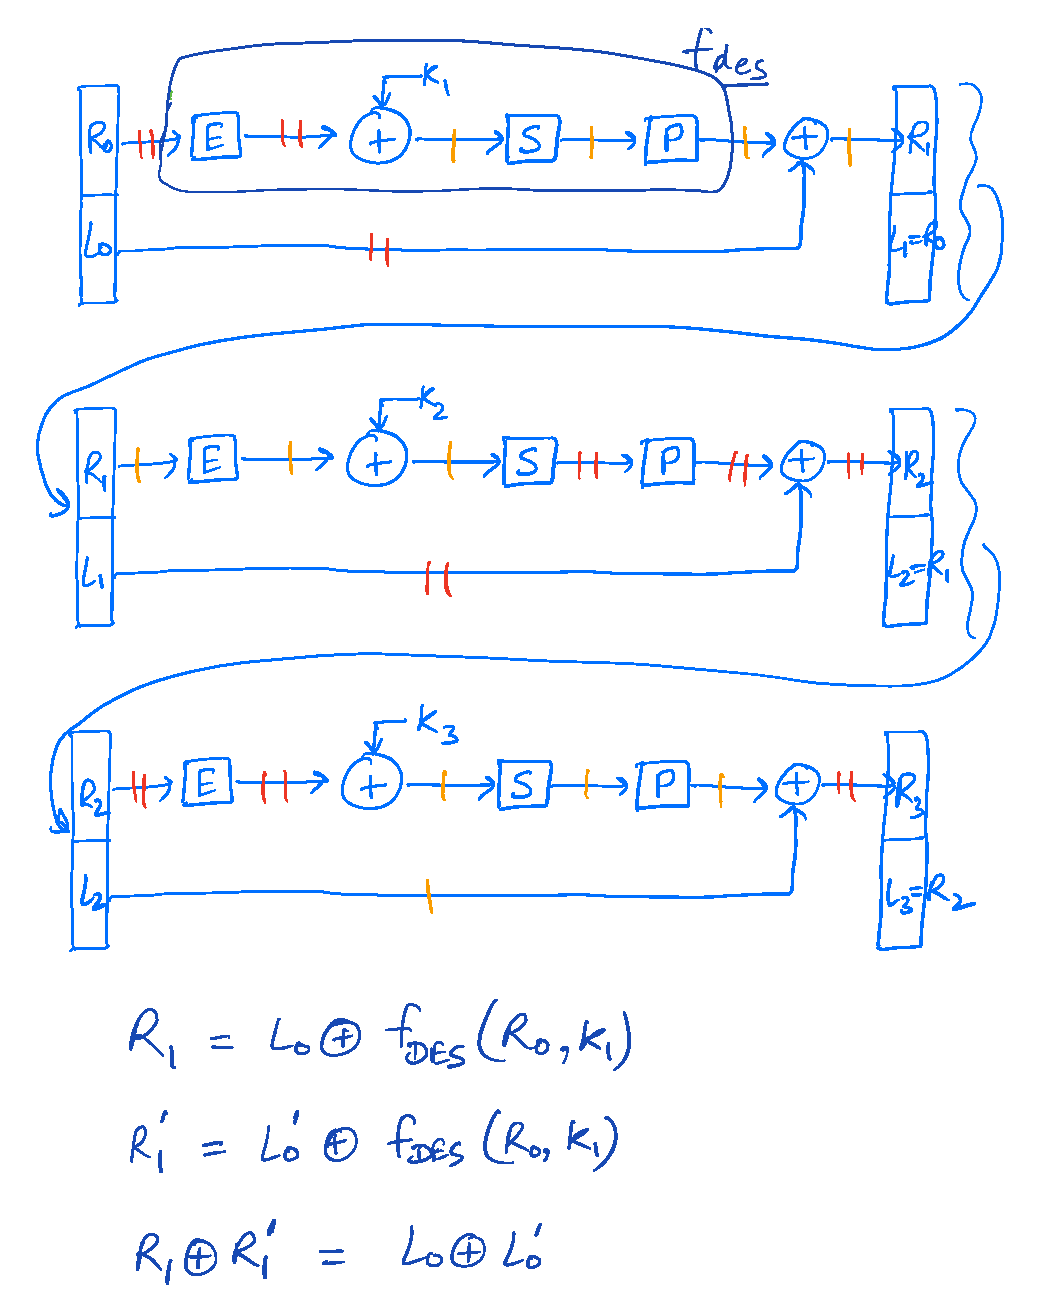
\includegraphics[scale=0.5]{des.pdf}
  \label{3-des}
  \caption{3 Round DES}
\end{figure}

Important points about the figure above:
\begin{itemize}
  \setlength\itemsep{0em}
  \item \textit{Double Red Line} implies we know both individual values of \textit{Differential Cryptanalysis}.
  \item \textit{Single Golden Line} implies we know the differential value of 2 inputs, not the individual values themselves.
  \item The pairs of inputs taken during Differential Cryptanalysis must have equal 32 bits on the right side.
\end{itemize}

Solving 3 Round DES:
\begin{enumerate}
  \setlength\itemsep{0em}
    \item We will start by figuring out the 48-bit Key for the 3rd Round.
    \item We know the differential value, just after and before the S-Boxes, thus, there will be 4 possible pairs of input values to the S-Box as studied in class.
    \item This narrows down the search for key over each 6 bits to 4 possibilities.
    \item We will pick another input here, take the intersection of possibilities and narrow down the key.
    \item After sufficient tries, we get the 48-bit 3rd round key.
    \item Now only 8 bits of the key remain, these can be easily brute-forced and figured out using the other round values.
\end{enumerate}

The code used in this part is as follows:
\begin{itemize}
  \setlength\itemsep{0em}
  \item \texttt{constants.py}: Contains the constants for the DES.
  \item \texttt{des.py}: Defines the DES Class encoding all the functions related to it.
  \item \texttt{utils.py}: Defines the common utility functions related to DES and Key generation.
  \item \texttt{break\_des.py}: Defines the main function which uses all the utilities and DES class to break the 3 Round DES according the steps described above.
  \item \texttt{generate\_input.py}: Generates a pair of input which have equal 32 bits on the right side.
\end{itemize}

The key retrieved for the 3rd round of the DES is as follows:
$$\texttt{[61, 28, 9, 54, 55, 9, 28, 51]}$$

here, each value represents the 6-bits of the 48-bit key. \newline 

After doing brute force on the remaining part of the key, we get the following value:
$$147$$

The Final Key (64-bit including the parity bits) for the DES is as follows:
$$0111101001011100001010000011011011110010011010100110101011101000$$

The encrypted password: \texttt{gnushmilfrplulktkrtrogltjojfqjpt} \newline
The decrypted password: \texttt{rirfiirqnujpopirgkholonsqntpkqqi}

\newpage
\section{Appendix}

This section explains each of the things used in between the solutions without proper explanation.

\subsection{Index of Coincidence} \label{ic}

The \textbf{Index of Coincidence} is a measure of how similar a frequency distribution is to the uniform distribution.
$$ I.C. = \frac{\sum_{i=A}^{i=Z} f_i(f_i-1)}{N(N-1)}$$

where $f_i$ is the count of letter $i$ (where $i = A,B,...,Z$) in the ciphertext, and $N$ is the total number of letters in the ciphertext. \newline

Important facts about the \textit{Index of Coincidence}:
\begin{itemize}
  \setlength\itemsep{0em}
    \item The \textit{Index of Coincidence} of valid English text is about $0.066$.
    \item The \textit{Index of Coincidence} for uniform distribution of English text is about $0.038$.
    \item The \textit{Index of Coincidence} remains the same for the ciphertext and plaintext if cipher is \textbf{Mono-alphabetic} (i.e. Substitution Cipher).
    \item The \textit{Index of Coincidence} of ciphertext is closer to uniform distribution if cipher is \textbf{Poly-alphabetic} (such as Vigenere Cipher).
\end{itemize}

We can get an approximate idea of what kind of cipher is used to generate the ciphertext by using the \textit{Index of Coincidence}.

\subsection{Chi-squared Statistic} \label{chi}
The \textbf{Chi-squared Statistic} is a measure of how similar two categorical probability distributions are. If the two distributions are identical, the chi-squared statistic is 0, if the distributions are very different, some higher number will result. The formula for the chi-squared statistic is:
$$\chi^2(C,E) = \sum_{i=A}^{i=Z}\frac{(C_i-E_i)^2}{E_i}$$

where $C_A$ is the count (not the probability) of letter $A$, and $E_A$ is the expected count of letter $A$. \newline

Important facts about the \textit{Chi-squared Statistic}:
\begin{itemize}
  \setlength\itemsep{0em}
  \item If the \textit{Chi-squared Statistic} of a ciphertext against \textit{uniform distribution} is very low (\textasciitilde 50 or less), then it is highly probable that the cipher is \textit{Poly-alphabetic}.
  \item If the \textit{Chi-squared Statistic} of a ciphertext against \textit{valid English text} is high and the cipher is \textit{Mono-alphabetic}, then it can be solved by trying keys and lowering it.
\end{itemize}

We can get an approximate idea of whether the cipher is \textit{Poly-alphabetic} or not by using \textit{Chi-squared Statistic}.

\subsection{Vigenere Cipher} \label{vc}
The Vigenere Cipher is a polyalphabetic substitution cipher. \newline

Suppose, the length of the encryption key is $k$, then the string formed by picking out each letter with a multiple of $k$ letters in between them will be a \textit{Caesar Cipher}. \newline

Since each such string is a \textit{Caesar Cipher}, the \textit{Index of Coincidence} of this string will be closer to that of valid English text rather than closer to uniform distribution. \newline

Using the above principle, we can crack the \textit{Vigenere Cipher}.

\end{document}
